\documentclass[conference]{IEEEtran}
\usepackage{graphicx}
\usepackage{amsmath,amssymb}
\usepackage{hyperref}
\usepackage{siunitx}
\usepackage{booktabs}
\usepackage{tikz}
\usetikzlibrary{positioning,arrows.meta} % ← これが必須(of を使う)

\tikzset{>=Latex, node/.style={draw, thick, minimum width=2.7cm, minimum height=0.9cm, align=center}}

\title{AITL on Space: A Robust Three-Layer Architecture with a Tri-NVM Hierarchy (SRAM / MRAM / FRAM) for Long-Duration Spacecraft Autonomy}

\author{%
  \IEEEauthorblockN{Shinichi Samizo}
  \IEEEauthorblockA{Independent Semiconductor Researcher\\
  Former Engineer at Seiko Epson Corporation\\
  Email: \href{mailto:shin3t72@gmail.com}{shin3t72@gmail.com}\\
  GitHub: \url{https://github.com/Samizo-AITL}}%
}

\begin{document}
\maketitle

\begin{abstract}
We propose \textbf{AITL on Space}, a three-layer control architecture (Robust Core, FSM Supervisor, AI Adaptor) implemented on a 22\,nm FDSOI SoC with a hardened \textbf{Tri-NVM hierarchy} (SRAM / MRAM / FRAM). The system targets ultra-robust autonomy under radiation, thermal cycling, and long-term drift. This paper outlines the architecture, state-space model (8--20\,D), H$\infty$ mixed-sensitivity design flow, and a verification pipeline from FPGA HIL to ASIC.
\end{abstract}

\section{Introduction}
Long-duration missions require high availability under TID/SEE and thermal cycles. Conventional PID+Flash architectures face reliability limits. We summarize related work and motivate AITL on Space.

\section{System Architecture}
AITL comprises: (i) Robust Core (H$\infty$/MPC/SMC), (ii) FSM Supervisor (Safe/Nominal/Recovery, FDI/FDII), and (iii) AI Adaptor for long-term re-identification. A \textbf{Tri-NVM hierarchy}---SRAM for execution, MRAM for logs/code (ECC+scrub, A/B slots), FRAM for safe boot---ensures persistence.

\begin{figure}[t]
  \centering
  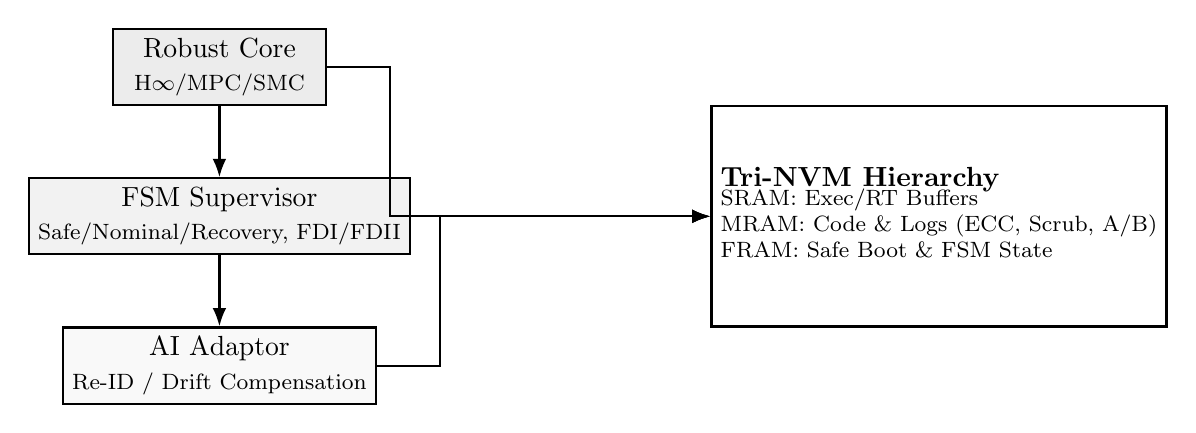
\begin{tikzpicture}[node distance=0.9cm]
    % 左の縦3層
    \node[node, fill=gray!15] (robust) {Robust Core\\{\footnotesize H$\infty$/MPC/SMC}};
    \node[node, fill=gray!10, below=of robust] (fsm) {FSM Supervisor\\{\footnotesize Safe/Nominal/Recovery, FDI/FDII}};
    \node[node, fill=gray!5,  below=of fsm] (ai) {AI Adaptor\\{\footnotesize Re-ID / Drift Compensation}};

    % 右ブロック(Tri-NVM)
    \node[node, fill=white, right=3.8cm of fsm, minimum width=3.7cm, minimum height=2.8cm, align=left] (nvm) {%
      \textbf{Tri-NVM Hierarchy}\\[-1mm]
      {\footnotesize \begin{tabular}{@{}l@{}}
        SRAM: Exec/RT Buffers\\
        MRAM: Code \& Logs (ECC, Scrub, A/B)\\
        FRAM: Safe Boot \& FSM State
      \end{tabular}}
    };

    % 矢印
    \draw[->, thick] (robust.east) -- ++(0.8,0) |- (nvm.west);
    \draw[->, thick] (fsm.east)   -- ++(0.8,0) |- (nvm.west);
    \draw[->, thick] (ai.east)    -- ++(0.8,0) |- (nvm.west);

    \draw[->, thick] (robust.south) -- (fsm.north);
    \draw[->, thick] (fsm.south) -- (ai.north);
  \end{tikzpicture}
  \caption{AITL on Space architecture with Robust Core, Supervisor FSM, AI Adaptor, and the Tri-NVM hierarchy.}
  \label{fig:arch_block}
\end{figure}

\section{Mathematical Model}
We use an 11D PoC plant that couples attitude (6), power bus (2), and thermal nodes (3). The discrete-time model is
\begin{align}
x_{k+1} &= A x_k + B u_k + E w_k, \quad
y_k = C x_k + D u_k + v_k.
\end{align}
Extensions scale to 20D with translational axes and bias states.

\begin{figure}[t]
  \centering
  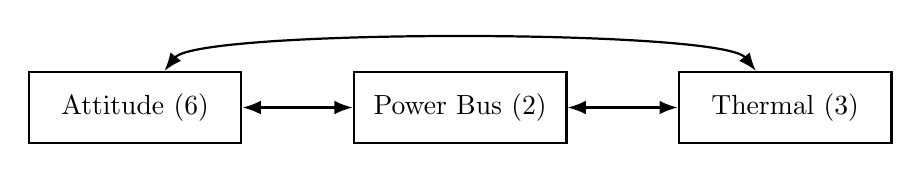
\begin{tikzpicture}
    \node[node] (att) {Attitude (6)};
    \node[node, right=1.4cm of att] (bus) {Power Bus (2)};
    \node[node, right=1.4cm of bus] (thermal) {Thermal (3)};
    \draw[<->, thick] (att) -- (bus);
    \draw[<->, thick] (bus) -- (thermal);
    \draw[<->, thick] (att) .. controls +(+0.8,1.0) and +(-0.8,1.0) .. (thermal);
  \end{tikzpicture}
  \caption{PoC 11D state-space model coupling attitude (6), power bus (2), and thermal nodes (3).}
  \label{fig:state_space}
\end{figure}

\section{H$\infty$ Mixed-Sensitivity Design}
Weights $(W_1,W_2,W_3)$ shape sensitivity, effort, and complementary sensitivity. EduController exports JSON plant/weights; AITL-H synthesizes output-feedback $K$ and fixed-point realization.

\section{Verification Pipeline}
FPGA HIL injects SEU bursts and sensor outages; metrics include safe-mode time ($\leq 1\,\mathrm{s}$), recovery rate ($\geq 99\%$), and ECC statistics. Physical design proceeds to 22FDX tape-out; SystemDK FEM closes thermal/packaging.

\begin{figure}[t]
  \centering
  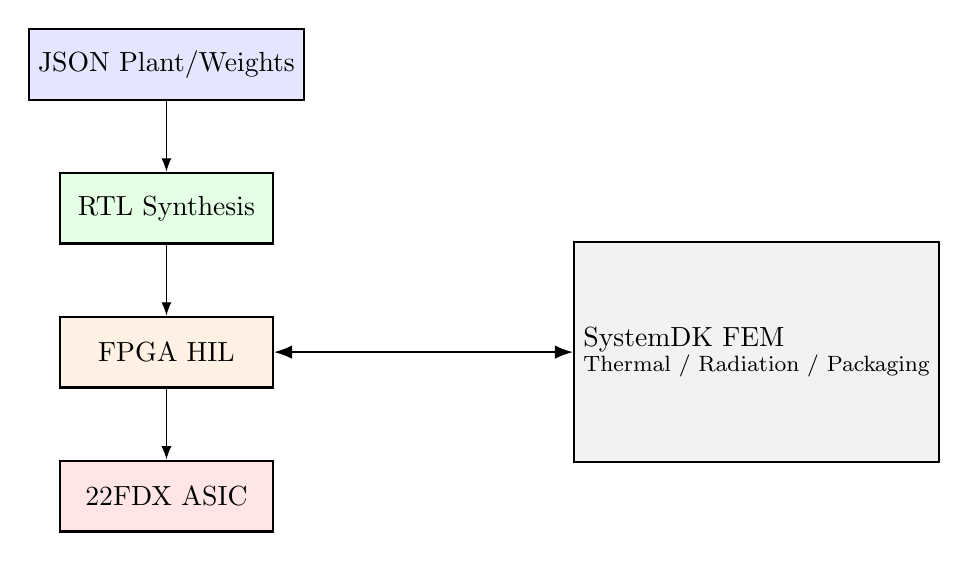
\begin{tikzpicture}[node distance=0.9cm]
    \node[node, fill=blue!10]   (json) {JSON Plant/Weights};
    \node[node, fill=green!10, below=of json] (rtl) {RTL Synthesis};
    \node[node, fill=orange!10, below=of rtl] (fpga) {FPGA HIL};
    \node[node, fill=red!10, below=of fpga] (asic) {22FDX ASIC};
    \node[node, fill=gray!10, right=3.8cm of fpga, minimum width=4.1cm, minimum height=2.8cm, align=left] (systemdk) {%
      SystemDK FEM\\[-1mm]
      {\footnotesize Thermal / Radiation / Packaging}
    };

    \draw[->] (json) -- (rtl);
    \draw[->] (rtl) -- (fpga);
    \draw[->] (fpga) -- (asic);
    \draw[<->, thick] (fpga.east) -- (systemdk.west);
  \end{tikzpicture}
  \caption{Verification pipeline from JSON design to RTL, FPGA HIL, and ASIC; SystemDK closes the loop with thermal and radiation scenarios.}
  \label{fig:pipeline}
\end{figure}

\section{Conclusion}
AITL on Space offers a practical path to resilient autonomy for deep-space missions.

\bibliographystyle{ieeetr}
\begin{thebibliography}{9}
\bibitem{hinf} Doyle, G. et al., \emph{Feedback Control Theory}.
\bibitem{fds} Colinge, J.-P., \emph{Silicon-on-Insulator Technology}.
\end{thebibliography}

\section*{Author Biography}
\textbf{Shinichi Samizo} received the M.S. degree in Electrical and Electronic
Engineering from Shinshu University, Japan. He worked at Seiko Epson
Corporation as an engineer in semiconductor memory and mixed-signal
device development, and contributed to inkjet MEMS actuators and
PrecisionCore printhead technology. He is currently an independent
semiconductor researcher focusing on process/device education, memory
architecture, and AI system integration. Contact:
\href{mailto:shin3t72@gmail.com}{shin3t72@gmail.com}.
\end{document}
